% Created by tikzDevice version 0.12.6 on 2026-08-03 03:40:42
% !TEX encoding = UTF-8 Unicode
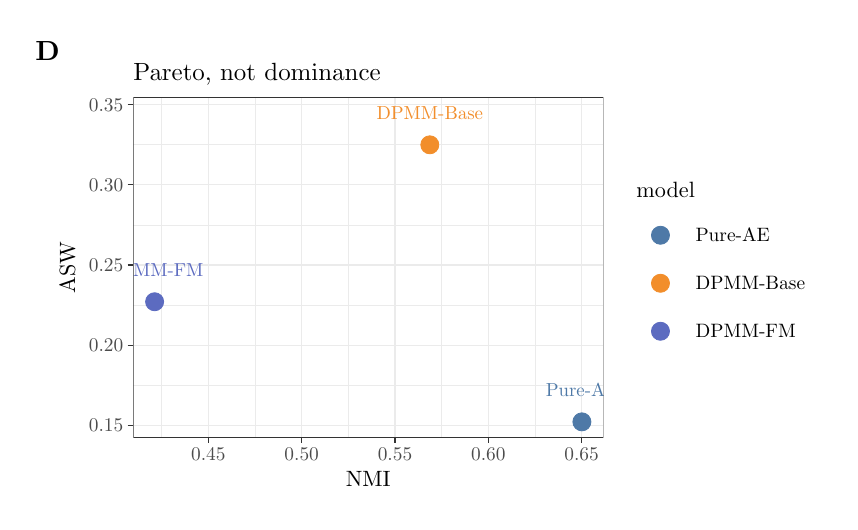
\begin{tikzpicture}[x=1pt,y=1pt]
\definecolor{fillColor}{RGB}{255,255,255}
\path[use as bounding box,fill=fillColor,fill opacity=0.00] (0,0) rectangle (289.70,171.36);
\begin{scope}
\path[clip] (  0.79,  1.87) rectangle (288.92,169.49);
\definecolor{drawColor}{RGB}{255,255,255}
\definecolor{fillColor}{RGB}{255,255,255}

\path[draw=drawColor,line width= 0.4pt,line join=round,line cap=round,fill=fillColor] (  0.79,  1.87) rectangle (288.92,169.49);
\end{scope}
\begin{scope}
\path[clip] ( 38.15, 23.34) rectangle (207.99,146.20);
\definecolor{fillColor}{RGB}{255,255,255}

\path[fill=fillColor] ( 38.15, 23.34) rectangle (207.99,146.20);
\definecolor{drawColor}{gray}{0.92}

\path[draw=drawColor,line width= 0.2pt,line join=round] ( 38.15, 42.17) --
	(207.99, 42.17);

\path[draw=drawColor,line width= 0.2pt,line join=round] ( 38.15, 71.13) --
	(207.99, 71.13);

\path[draw=drawColor,line width= 0.2pt,line join=round] ( 38.15,100.09) --
	(207.99,100.09);

\path[draw=drawColor,line width= 0.2pt,line join=round] ( 38.15,129.05) --
	(207.99,129.05);

\path[draw=drawColor,line width= 0.2pt,line join=round] ( 48.43, 23.34) --
	( 48.43,146.20);

\path[draw=drawColor,line width= 0.2pt,line join=round] ( 82.15, 23.34) --
	( 82.15,146.20);

\path[draw=drawColor,line width= 0.2pt,line join=round] (115.87, 23.34) --
	(115.87,146.20);

\path[draw=drawColor,line width= 0.2pt,line join=round] (149.59, 23.34) --
	(149.59,146.20);

\path[draw=drawColor,line width= 0.2pt,line join=round] (183.31, 23.34) --
	(183.31,146.20);

\path[draw=drawColor,line width= 0.4pt,line join=round] ( 38.15, 27.69) --
	(207.99, 27.69);

\path[draw=drawColor,line width= 0.4pt,line join=round] ( 38.15, 56.65) --
	(207.99, 56.65);

\path[draw=drawColor,line width= 0.4pt,line join=round] ( 38.15, 85.61) --
	(207.99, 85.61);

\path[draw=drawColor,line width= 0.4pt,line join=round] ( 38.15,114.57) --
	(207.99,114.57);

\path[draw=drawColor,line width= 0.4pt,line join=round] ( 38.15,143.53) --
	(207.99,143.53);

\path[draw=drawColor,line width= 0.4pt,line join=round] ( 65.29, 23.34) --
	( 65.29,146.20);

\path[draw=drawColor,line width= 0.4pt,line join=round] ( 99.01, 23.34) --
	( 99.01,146.20);

\path[draw=drawColor,line width= 0.4pt,line join=round] (132.73, 23.34) --
	(132.73,146.20);

\path[draw=drawColor,line width= 0.4pt,line join=round] (166.45, 23.34) --
	(166.45,146.20);

\path[draw=drawColor,line width= 0.4pt,line join=round] (200.17, 23.34) --
	(200.17,146.20);
\definecolor{drawColor}{RGB}{242,142,43}
\definecolor{fillColor}{RGB}{242,142,43}

\path[draw=drawColor,line width= 0.3pt,line join=round,line cap=round,fill=fillColor] (145.31,129.03) circle (  3.26);
\definecolor{drawColor}{RGB}{92,107,192}
\definecolor{fillColor}{RGB}{92,107,192}

\path[draw=drawColor,line width= 0.3pt,line join=round,line cap=round,fill=fillColor] ( 45.87, 72.32) circle (  3.26);
\definecolor{drawColor}{RGB}{78,121,167}
\definecolor{fillColor}{RGB}{78,121,167}

\path[draw=drawColor,line width= 0.3pt,line join=round,line cap=round,fill=fillColor] (200.27, 28.92) circle (  3.26);
\definecolor{drawColor}{RGB}{242,142,43}

\node[text=drawColor,anchor=base,inner sep=0pt, outer sep=0pt, scale=  0.68] at (145.31,138.26) {DPMM-Base};
\definecolor{drawColor}{RGB}{92,107,192}

\node[text=drawColor,anchor=base,inner sep=0pt, outer sep=0pt, scale=  0.68] at ( 45.87, 81.55) {DPMM-FM};
\definecolor{drawColor}{RGB}{78,121,167}

\node[text=drawColor,anchor=base,inner sep=0pt, outer sep=0pt, scale=  0.68] at (200.27, 38.15) {Pure-AE};
\definecolor{drawColor}{gray}{0.20}

\path[draw=drawColor,line width= 0.4pt,line join=round,line cap=round] ( 38.15, 23.34) rectangle (207.99,146.20);
\end{scope}
\begin{scope}
\path[clip] (  0.00,  0.00) rectangle (289.70,171.36);
\definecolor{drawColor}{gray}{0.30}

\node[text=drawColor,anchor=base east,inner sep=0pt, outer sep=0pt, scale=  0.70] at ( 34.55, 25.28) {0.15};

\node[text=drawColor,anchor=base east,inner sep=0pt, outer sep=0pt, scale=  0.70] at ( 34.55, 54.24) {0.20};

\node[text=drawColor,anchor=base east,inner sep=0pt, outer sep=0pt, scale=  0.70] at ( 34.55, 83.20) {0.25};

\node[text=drawColor,anchor=base east,inner sep=0pt, outer sep=0pt, scale=  0.70] at ( 34.55,112.16) {0.30};

\node[text=drawColor,anchor=base east,inner sep=0pt, outer sep=0pt, scale=  0.70] at ( 34.55,141.12) {0.35};
\end{scope}
\begin{scope}
\path[clip] (  0.00,  0.00) rectangle (289.70,171.36);
\definecolor{drawColor}{gray}{0.20}

\path[draw=drawColor,line width= 0.4pt,line join=round] ( 36.15, 27.69) --
	( 38.15, 27.69);

\path[draw=drawColor,line width= 0.4pt,line join=round] ( 36.15, 56.65) --
	( 38.15, 56.65);

\path[draw=drawColor,line width= 0.4pt,line join=round] ( 36.15, 85.61) --
	( 38.15, 85.61);

\path[draw=drawColor,line width= 0.4pt,line join=round] ( 36.15,114.57) --
	( 38.15,114.57);

\path[draw=drawColor,line width= 0.4pt,line join=round] ( 36.15,143.53) --
	( 38.15,143.53);
\end{scope}
\begin{scope}
\path[clip] (  0.00,  0.00) rectangle (289.70,171.36);
\definecolor{drawColor}{gray}{0.20}

\path[draw=drawColor,line width= 0.4pt,line join=round] ( 65.29, 21.34) --
	( 65.29, 23.34);

\path[draw=drawColor,line width= 0.4pt,line join=round] ( 99.01, 21.34) --
	( 99.01, 23.34);

\path[draw=drawColor,line width= 0.4pt,line join=round] (132.73, 21.34) --
	(132.73, 23.34);

\path[draw=drawColor,line width= 0.4pt,line join=round] (166.45, 21.34) --
	(166.45, 23.34);

\path[draw=drawColor,line width= 0.4pt,line join=round] (200.17, 21.34) --
	(200.17, 23.34);
\end{scope}
\begin{scope}
\path[clip] (  0.00,  0.00) rectangle (289.70,171.36);
\definecolor{drawColor}{gray}{0.30}

\node[text=drawColor,anchor=base,inner sep=0pt, outer sep=0pt, scale=  0.70] at ( 65.29, 14.92) {0.45};

\node[text=drawColor,anchor=base,inner sep=0pt, outer sep=0pt, scale=  0.70] at ( 99.01, 14.92) {0.50};

\node[text=drawColor,anchor=base,inner sep=0pt, outer sep=0pt, scale=  0.70] at (132.73, 14.92) {0.55};

\node[text=drawColor,anchor=base,inner sep=0pt, outer sep=0pt, scale=  0.70] at (166.45, 14.92) {0.60};

\node[text=drawColor,anchor=base,inner sep=0pt, outer sep=0pt, scale=  0.70] at (200.17, 14.92) {0.65};
\end{scope}
\begin{scope}
\path[clip] (  0.00,  0.00) rectangle (289.70,171.36);
\definecolor{drawColor}{RGB}{0,0,0}

\node[text=drawColor,anchor=base,inner sep=0pt, outer sep=0pt, scale=  0.80] at (123.07,  5.64) {NMI};
\end{scope}
\begin{scope}
\path[clip] (  0.00,  0.00) rectangle (289.70,171.36);
\definecolor{drawColor}{RGB}{0,0,0}

\node[text=drawColor,rotate= 90.00,anchor=base,inner sep=0pt, outer sep=0pt, scale=  0.80] at ( 17.12, 84.77) {ASW};
\end{scope}
\begin{scope}
\path[clip] (  0.00,  0.00) rectangle (289.70,171.36);
\definecolor{fillColor}{RGB}{255,255,255}

\path[fill=fillColor] (215.99, 48.98) rectangle (286.92,120.55);
\end{scope}
\begin{scope}
\path[clip] (  0.00,  0.00) rectangle (289.70,171.36);
\definecolor{drawColor}{RGB}{0,0,0}

\node[text=drawColor,anchor=base west,inner sep=0pt, outer sep=0pt, scale=  0.80] at (219.99,110.03) {model};
\end{scope}
\begin{scope}
\path[clip] (  0.00,  0.00) rectangle (289.70,171.36);
\definecolor{fillColor}{RGB}{255,255,255}

\path[fill=fillColor] (219.99, 87.67) rectangle (237.33,105.02);
\definecolor{drawColor}{RGB}{78,121,167}
\definecolor{fillColor}{RGB}{78,121,167}

\path[draw=drawColor,line width= 0.3pt,line join=round,line cap=round,fill=fillColor] (228.66, 96.35) circle (  3.26);
\end{scope}
\begin{scope}
\path[clip] (  0.00,  0.00) rectangle (289.70,171.36);
\definecolor{fillColor}{RGB}{255,255,255}

\path[fill=fillColor] (219.99, 70.33) rectangle (237.33, 87.67);
\definecolor{drawColor}{RGB}{242,142,43}
\definecolor{fillColor}{RGB}{242,142,43}

\path[draw=drawColor,line width= 0.3pt,line join=round,line cap=round,fill=fillColor] (228.66, 79.00) circle (  3.26);
\end{scope}
\begin{scope}
\path[clip] (  0.00,  0.00) rectangle (289.70,171.36);
\definecolor{fillColor}{RGB}{255,255,255}

\path[fill=fillColor] (219.99, 52.98) rectangle (237.33, 70.33);
\definecolor{drawColor}{RGB}{92,107,192}
\definecolor{fillColor}{RGB}{92,107,192}

\path[draw=drawColor,line width= 0.3pt,line join=round,line cap=round,fill=fillColor] (228.66, 61.66) circle (  3.26);
\end{scope}
\begin{scope}
\path[clip] (  0.00,  0.00) rectangle (289.70,171.36);
\definecolor{drawColor}{RGB}{0,0,0}

\node[text=drawColor,anchor=base west,inner sep=0pt, outer sep=0pt, scale=  0.70] at (241.33, 93.93) {Pure-AE};
\end{scope}
\begin{scope}
\path[clip] (  0.00,  0.00) rectangle (289.70,171.36);
\definecolor{drawColor}{RGB}{0,0,0}

\node[text=drawColor,anchor=base west,inner sep=0pt, outer sep=0pt, scale=  0.70] at (241.33, 76.59) {DPMM-Base};
\end{scope}
\begin{scope}
\path[clip] (  0.00,  0.00) rectangle (289.70,171.36);
\definecolor{drawColor}{RGB}{0,0,0}

\node[text=drawColor,anchor=base west,inner sep=0pt, outer sep=0pt, scale=  0.70] at (241.33, 59.25) {DPMM-FM};
\end{scope}
\begin{scope}
\path[clip] (  0.00,  0.00) rectangle (289.70,171.36);
\definecolor{drawColor}{RGB}{0,0,0}

\node[text=drawColor,anchor=base west,inner sep=0pt, outer sep=0pt, scale=  0.90] at ( 38.15,152.18) {Pareto, not dominance};
\end{scope}
\begin{scope}
\path[clip] (  0.00,  0.00) rectangle (289.70,171.36);
\definecolor{drawColor}{RGB}{0,0,0}

\node[text=drawColor,anchor=base,inner sep=0pt, outer sep=0pt, scale=  1.00] at (  7.20,159.49) {\bfseries D};
\end{scope}
\end{tikzpicture}
